\documentclass[tikz,border=3pt]{standalone}
\usepackage[utf8]{inputenc}
\usepackage[T1]{fontenc}
\usepackage{libertinus}
\usepackage{amsmath,amssymb}
\usetikzlibrary{arrows.meta,calc,patterns,decorations.pathmorphing,decorations.markings,decorations.pathreplacing,bending}
\definecolor{UGblue}{RGB}{0,51,102}
\newcommand{\dbar}{\mathchar'26\mkern-12mu d}
\tikzset{
  >=Stealth,
  every node/.style={font=\small},
  caja/.style={draw,line width=0.9pt},
  pared/.style={draw,line width=1.6pt},
  ejes/.style={->,line width=0.8pt},
  adia/.style={draw,pattern=north east lines,pattern color=black!70,line width=0.5pt},
  gas/.style={fill=UGblue!8},
  punto/.style={fill,circle,inner sep=1.3pt},
  onda/.style={decorate,decoration={snake,amplitude=1.1pt,segment length=5pt,post length=3pt,pre length=0pt}},
}
\begin{document}
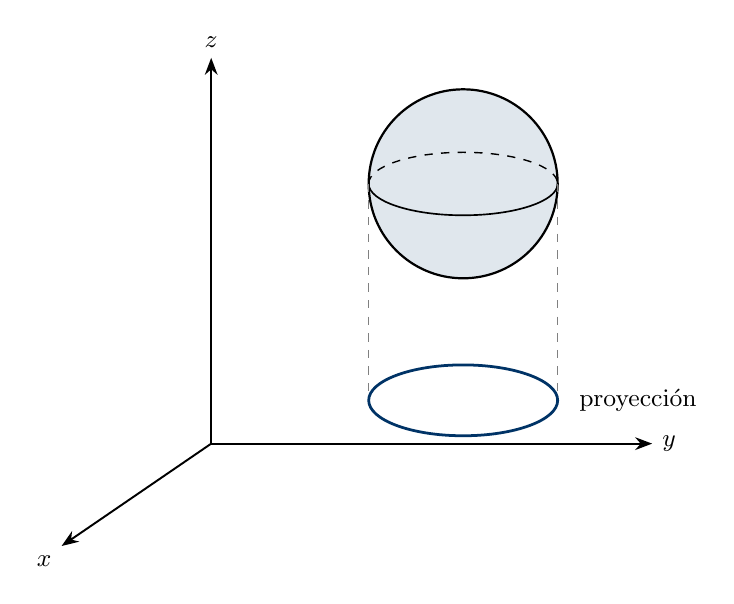
\begin{tikzpicture}
  \draw[->,line width=0.7pt] (0,0) -- (5.6,0) node[right] {$y$};
  \draw[->,line width=0.7pt] (0,0) -- (0,4.9) node[above] {$z$};
  \draw[->,line width=0.7pt] (0,0) -- (-1.9,-1.3) node[below left] {$x$};
  % esfera
  \fill[UGblue!12] (3.2,3.3) circle (1.2);
  \draw[line width=0.8pt] (3.2,3.3) circle (1.2);
  \draw[dashed,line width=0.5pt] (2,3.3) arc (180:0:1.2 and 0.4);
  \draw[line width=0.6pt] (2,3.3) arc (180:360:1.2 and 0.4);
  % proyección
  \draw[dashed,gray,line width=0.5pt] (2,3.3) -- (2,0.55);
  \draw[dashed,gray,line width=0.5pt] (4.4,3.3) -- (4.4,0.55);
  \draw[UGblue,line width=1pt] (3.2,0.55) ellipse (1.2 and 0.45);
  \node[right] at (4.55,0.55) {proyección};
\end{tikzpicture}
\end{document}
